\documentclass[]{article}
\usepackage{lmodern}
\usepackage{amssymb,amsmath}
\usepackage{ifxetex,ifluatex}
\usepackage{fixltx2e} % provides \textsubscript
\ifnum 0\ifxetex 1\fi\ifluatex 1\fi=0 % if pdftex
  \usepackage[T1]{fontenc}
  \usepackage[utf8]{inputenc}
\else % if luatex or xelatex
  \ifxetex
    \usepackage{mathspec}
  \else
    \usepackage{fontspec}
  \fi
  \defaultfontfeatures{Ligatures=TeX,Scale=MatchLowercase}
\fi
% use upquote if available, for straight quotes in verbatim environments
\IfFileExists{upquote.sty}{\usepackage{upquote}}{}
% use microtype if available
\IfFileExists{microtype.sty}{%
\usepackage{microtype}
\UseMicrotypeSet[protrusion]{basicmath} % disable protrusion for tt fonts
}{}
\usepackage[margin=1in]{geometry}
\usepackage{hyperref}
\hypersetup{unicode=true,
            pdftitle={Assignment 11},
            pdfauthor={Christophe Hunt},
            pdfborder={0 0 0},
            breaklinks=true}
\urlstyle{same}  % don't use monospace font for urls
\usepackage{color}
\usepackage{fancyvrb}
\newcommand{\VerbBar}{|}
\newcommand{\VERB}{\Verb[commandchars=\\\{\}]}
\DefineVerbatimEnvironment{Highlighting}{Verbatim}{commandchars=\\\{\}}
% Add ',fontsize=\small' for more characters per line
\usepackage{framed}
\definecolor{shadecolor}{RGB}{248,248,248}
\newenvironment{Shaded}{\begin{snugshade}}{\end{snugshade}}
\newcommand{\KeywordTok}[1]{\textcolor[rgb]{0.13,0.29,0.53}{\textbf{{#1}}}}
\newcommand{\DataTypeTok}[1]{\textcolor[rgb]{0.13,0.29,0.53}{{#1}}}
\newcommand{\DecValTok}[1]{\textcolor[rgb]{0.00,0.00,0.81}{{#1}}}
\newcommand{\BaseNTok}[1]{\textcolor[rgb]{0.00,0.00,0.81}{{#1}}}
\newcommand{\FloatTok}[1]{\textcolor[rgb]{0.00,0.00,0.81}{{#1}}}
\newcommand{\ConstantTok}[1]{\textcolor[rgb]{0.00,0.00,0.00}{{#1}}}
\newcommand{\CharTok}[1]{\textcolor[rgb]{0.31,0.60,0.02}{{#1}}}
\newcommand{\SpecialCharTok}[1]{\textcolor[rgb]{0.00,0.00,0.00}{{#1}}}
\newcommand{\StringTok}[1]{\textcolor[rgb]{0.31,0.60,0.02}{{#1}}}
\newcommand{\VerbatimStringTok}[1]{\textcolor[rgb]{0.31,0.60,0.02}{{#1}}}
\newcommand{\SpecialStringTok}[1]{\textcolor[rgb]{0.31,0.60,0.02}{{#1}}}
\newcommand{\ImportTok}[1]{{#1}}
\newcommand{\CommentTok}[1]{\textcolor[rgb]{0.56,0.35,0.01}{\textit{{#1}}}}
\newcommand{\DocumentationTok}[1]{\textcolor[rgb]{0.56,0.35,0.01}{\textbf{\textit{{#1}}}}}
\newcommand{\AnnotationTok}[1]{\textcolor[rgb]{0.56,0.35,0.01}{\textbf{\textit{{#1}}}}}
\newcommand{\CommentVarTok}[1]{\textcolor[rgb]{0.56,0.35,0.01}{\textbf{\textit{{#1}}}}}
\newcommand{\OtherTok}[1]{\textcolor[rgb]{0.56,0.35,0.01}{{#1}}}
\newcommand{\FunctionTok}[1]{\textcolor[rgb]{0.00,0.00,0.00}{{#1}}}
\newcommand{\VariableTok}[1]{\textcolor[rgb]{0.00,0.00,0.00}{{#1}}}
\newcommand{\ControlFlowTok}[1]{\textcolor[rgb]{0.13,0.29,0.53}{\textbf{{#1}}}}
\newcommand{\OperatorTok}[1]{\textcolor[rgb]{0.81,0.36,0.00}{\textbf{{#1}}}}
\newcommand{\BuiltInTok}[1]{{#1}}
\newcommand{\ExtensionTok}[1]{{#1}}
\newcommand{\PreprocessorTok}[1]{\textcolor[rgb]{0.56,0.35,0.01}{\textit{{#1}}}}
\newcommand{\AttributeTok}[1]{\textcolor[rgb]{0.77,0.63,0.00}{{#1}}}
\newcommand{\RegionMarkerTok}[1]{{#1}}
\newcommand{\InformationTok}[1]{\textcolor[rgb]{0.56,0.35,0.01}{\textbf{\textit{{#1}}}}}
\newcommand{\WarningTok}[1]{\textcolor[rgb]{0.56,0.35,0.01}{\textbf{\textit{{#1}}}}}
\newcommand{\AlertTok}[1]{\textcolor[rgb]{0.94,0.16,0.16}{{#1}}}
\newcommand{\ErrorTok}[1]{\textcolor[rgb]{0.64,0.00,0.00}{\textbf{{#1}}}}
\newcommand{\NormalTok}[1]{{#1}}
\usepackage{graphicx,grffile}
\makeatletter
\def\maxwidth{\ifdim\Gin@nat@width>\linewidth\linewidth\else\Gin@nat@width\fi}
\def\maxheight{\ifdim\Gin@nat@height>\textheight\textheight\else\Gin@nat@height\fi}
\makeatother
% Scale images if necessary, so that they will not overflow the page
% margins by default, and it is still possible to overwrite the defaults
% using explicit options in \includegraphics[width, height, ...]{}
\setkeys{Gin}{width=\maxwidth,height=\maxheight,keepaspectratio}
\IfFileExists{parskip.sty}{%
\usepackage{parskip}
}{% else
\setlength{\parindent}{0pt}
\setlength{\parskip}{6pt plus 2pt minus 1pt}
}
\setlength{\emergencystretch}{3em}  % prevent overfull lines
\providecommand{\tightlist}{%
  \setlength{\itemsep}{0pt}\setlength{\parskip}{0pt}}
\setcounter{secnumdepth}{5}
% Redefines (sub)paragraphs to behave more like sections
\ifx\paragraph\undefined\else
\let\oldparagraph\paragraph
\renewcommand{\paragraph}[1]{\oldparagraph{#1}\mbox{}}
\fi
\ifx\subparagraph\undefined\else
\let\oldsubparagraph\subparagraph
\renewcommand{\subparagraph}[1]{\oldsubparagraph{#1}\mbox{}}
\fi

%%% Use protect on footnotes to avoid problems with footnotes in titles
\let\rmarkdownfootnote\footnote%
\def\footnote{\protect\rmarkdownfootnote}

%%% Change title format to be more compact
\usepackage{titling}

% Create subtitle command for use in maketitle
\newcommand{\subtitle}[1]{
  \posttitle{
    \begin{center}\large#1\end{center}
    }
}

\setlength{\droptitle}{-2em}
  \title{Assignment 11}
  \pretitle{\vspace{\droptitle}\centering\huge}
  \posttitle{\par}
  \author{Christophe Hunt}
  \preauthor{\centering\large\emph}
  \postauthor{\par}
  \predate{\centering\large\emph}
  \postdate{\par}
  \date{April 23, 2017}

\usepackage{relsize}
\usepackage{setspace}
\usepackage{amsmath,amsfonts,amsthm}
\usepackage[sfdefault]{roboto}
\usepackage[T1]{fontenc}
\usepackage{float}
\usepackage{multirow}
\usepackage{mathtools}
\usepackage{tikz}

\begin{document}
\maketitle

{
\setcounter{tocdepth}{2}
\tableofcontents
}
Using R's lm function, perform regression analysis and measure the
significance of the independent variables for the following two data
sets.

In the first case, you are evaluating the statement that we hear that
Maximum Heart Rate of a person is related to their age by the following
equation:

MaxHR = 220 - Age

You have been given the following sample:

Age 18 23 25 35 65 54 34 56 72 19 23 42 18 39 37 \newline
MaxHR 202 186 187 180 156 169 174 172 153 199 193 174 198 183 178

Perform a linear regression analysis fitting the Max Heart Rate to Age
using the lm function in R. What is the resulting equation?

\begin{Shaded}
\begin{Highlighting}[]
\KeywordTok{library}\NormalTok{(stargazer)}
\NormalTok{Age <-}\StringTok{ }\KeywordTok{c}\NormalTok{(}\DecValTok{18}\NormalTok{, }\DecValTok{23}\NormalTok{, }\DecValTok{25}\NormalTok{, }\DecValTok{35}\NormalTok{, }\DecValTok{65}\NormalTok{, }\DecValTok{54}\NormalTok{, }\DecValTok{34}\NormalTok{, }\DecValTok{56}\NormalTok{, }\DecValTok{72}\NormalTok{, }\DecValTok{19}\NormalTok{, }\DecValTok{23}\NormalTok{, }\DecValTok{42}\NormalTok{, }\DecValTok{18}\NormalTok{, }\DecValTok{39}\NormalTok{, }\DecValTok{37}\NormalTok{)}
\NormalTok{MaxHR <-}\StringTok{ }\KeywordTok{c}\NormalTok{(}\DecValTok{202}\NormalTok{, }\DecValTok{186}\NormalTok{, }\DecValTok{187}\NormalTok{, }\DecValTok{180}\NormalTok{, }\DecValTok{156}\NormalTok{, }\DecValTok{169}\NormalTok{, }\DecValTok{174}\NormalTok{, }\DecValTok{172}\NormalTok{, }\DecValTok{153}\NormalTok{, }\DecValTok{199}\NormalTok{, }\DecValTok{193}\NormalTok{, }\DecValTok{174}\NormalTok{, }\DecValTok{198}\NormalTok{, }\DecValTok{183}\NormalTok{, }\DecValTok{178}\NormalTok{)}
\NormalTok{fit <-}\StringTok{ }\KeywordTok{lm}\NormalTok{(MaxHR~Age)}
\KeywordTok{stargazer}\NormalTok{(fit, }\DataTypeTok{header =} \OtherTok{FALSE}\NormalTok{)}
\end{Highlighting}
\end{Shaded}

\begin{table}[!htbp] \centering 
  \caption{} 
  \label{} 
\begin{tabular}{@{\extracolsep{5pt}}lc} 
\\[-1.8ex]\hline 
\hline \\[-1.8ex] 
 & \multicolumn{1}{c}{\textit{Dependent variable:}} \\ 
\cline{2-2} 
\\[-1.8ex] & MaxHR \\ 
\hline \\[-1.8ex] 
 Age & $-$0.798$^{***}$ \\ 
  & (0.070) \\ 
  & \\ 
 Constant & 210.048$^{***}$ \\ 
  & (2.867) \\ 
  & \\ 
\hline \\[-1.8ex] 
Observations & 15 \\ 
R$^{2}$ & 0.909 \\ 
Adjusted R$^{2}$ & 0.902 \\ 
Residual Std. Error & 4.578 (df = 13) \\ 
F Statistic & 130.009$^{***}$ (df = 1; 13) \\ 
\hline 
\hline \\[-1.8ex] 
\textit{Note:}  & \multicolumn{1}{r}{$^{*}$p$<$0.1; $^{**}$p$<$0.05; $^{***}$p$<$0.01} \\ 
\end{tabular} 
\end{table}

Is the effect of Age on Max HR significant?

\begin{quote}
Yes, the effect of Age on MaxH is significant. We see the
p\textless{}0.01 for Age which indicates that it is indeed signficiant.
We would say anything with a p\textless{}0.05 is typically significant,
depending on the situation.
\end{quote}

\newpage

What is the significance level?

\begin{quote}
The signficance level is p\textless{}0.01, the exact value is as
follows.
\end{quote}

\begin{Shaded}
\begin{Highlighting}[]
\KeywordTok{options}\NormalTok{(}\DataTypeTok{scipen =} \DecValTok{999}\NormalTok{)}
\NormalTok{x <-}\StringTok{ }\KeywordTok{anova}\NormalTok{(fit)}
\NormalTok{x$}\StringTok{`}\DataTypeTok{Pr(>F)}\StringTok{`}\NormalTok{[}\DecValTok{1}\NormalTok{]}
\end{Highlighting}
\end{Shaded}

\begin{verbatim}
## [1] 0.00000003847987
\end{verbatim}

Please also plot the fitted relationship between Max HR and Age.

\begin{Shaded}
\begin{Highlighting}[]
\KeywordTok{plot}\NormalTok{(MaxHR~Age)}
\end{Highlighting}
\end{Shaded}

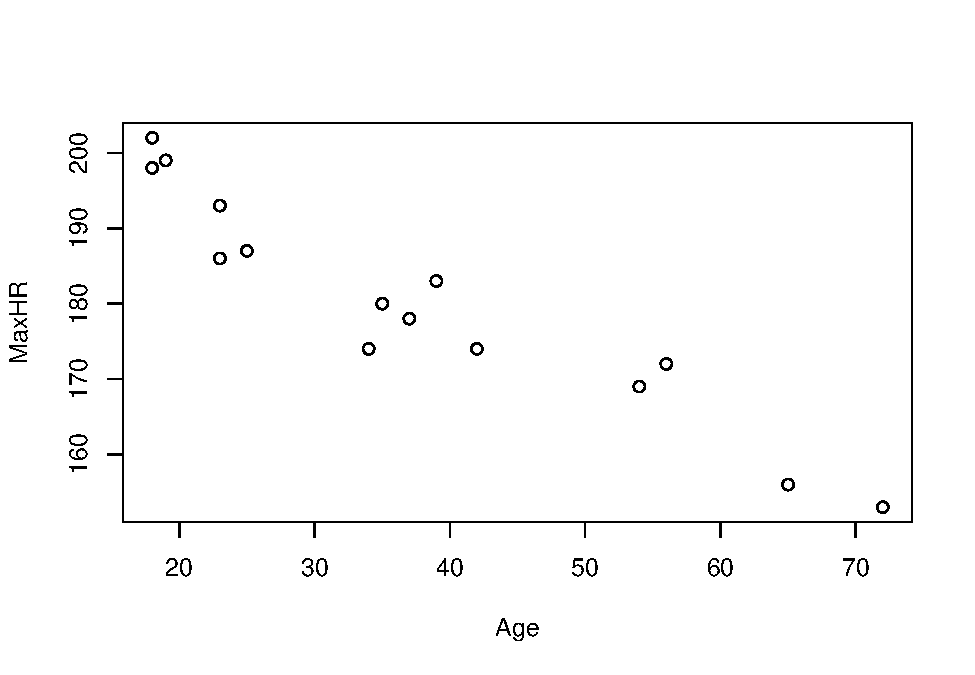
\includegraphics{CHunt_Assign11_files/figure-latex/unnamed-chunk-4-1.pdf}

\newpage

Using the Auto data set from Assignment 5 (also attached here) perform a
Linear Regression analysis using mpg as the dependent variable and the
other 4 (displacement, horse-power, weight, acceleration) as independent
variables.

What is the final linear regression fit equation?

\begin{Shaded}
\begin{Highlighting}[]
\KeywordTok{library}\NormalTok{(tidyverse)}
\NormalTok{df <-}\StringTok{ }\KeywordTok{as_tibble}\NormalTok{(}\KeywordTok{read.table}\NormalTok{(}\KeywordTok{paste0}\NormalTok{(}\StringTok{"https://raw.githubusercontent.com"}\NormalTok{,}
                                 \StringTok{"/ChristopheHunt/MSDA---Coursework"}\NormalTok{,}
                                 \StringTok{"/master/Data%20605/Assignment%2011/"}\NormalTok{,}
                                 \StringTok{"auto-mpg.data"}\NormalTok{)))}
\KeywordTok{colnames}\NormalTok{(df) <-}\StringTok{ }\KeywordTok{c}\NormalTok{(}\StringTok{"displacement"}\NormalTok{, }\StringTok{"horsepower"}\NormalTok{, }\StringTok{"weight"}\NormalTok{, }\StringTok{"acceleration"}\NormalTok{, }\StringTok{"mpg"}\NormalTok{)}
\end{Highlighting}
\end{Shaded}

\begin{Shaded}
\begin{Highlighting}[]
\NormalTok{fit <-}\StringTok{ }\KeywordTok{lm}\NormalTok{(}\DataTypeTok{data =} \NormalTok{df, }\DataTypeTok{formula =} \NormalTok{(mpg ~}\StringTok{ }\NormalTok{displacement +}\StringTok{  }\NormalTok{horsepower +}
\StringTok{                                  }\NormalTok{weight +}\StringTok{ }\NormalTok{acceleration))}
\KeywordTok{stargazer}\NormalTok{(fit, }\DataTypeTok{header =} \OtherTok{FALSE}\NormalTok{)}
\end{Highlighting}
\end{Shaded}

\begin{table}[!htbp] \centering 
  \caption{} 
  \label{} 
\begin{tabular}{@{\extracolsep{5pt}}lc} 
\\[-1.8ex]\hline 
\hline \\[-1.8ex] 
 & \multicolumn{1}{c}{\textit{Dependent variable:}} \\ 
\cline{2-2} 
\\[-1.8ex] & mpg \textasciitilde displacement + horsepower + weight + acceleration \\ 
\hline \\[-1.8ex] 
 displacement & $-$0.006 \\ 
  & (0.007) \\ 
  & \\ 
 horsepower & $-$0.044$^{***}$ \\ 
  & (0.017) \\ 
  & \\ 
 weight & $-$0.005$^{***}$ \\ 
  & (0.001) \\ 
  & \\ 
 acceleration & $-$0.023 \\ 
  & (0.126) \\ 
  & \\ 
 Constant & 45.251$^{***}$ \\ 
  & (2.456) \\ 
  & \\ 
\hline \\[-1.8ex] 
Observations & 392 \\ 
R$^{2}$ & 0.707 \\ 
Adjusted R$^{2}$ & 0.704 \\ 
Residual Std. Error & 4.247 (df = 387) \\ 
F Statistic & 233.434$^{***}$ (df = 4; 387) \\ 
\hline 
\hline \\[-1.8ex] 
\textit{Note:}  & \multicolumn{1}{r}{$^{*}$p$<$0.1; $^{**}$p$<$0.05; $^{***}$p$<$0.01} \\ 
\end{tabular} 
\end{table}

\newpage

Which of the 4 independent variables have a significant impact on mpg?

\begin{quote}
Horsepower and weight have a significant impact on mpg. It is unlikely
that their values have an impact on mpg merely by chance.
\end{quote}

What are their corresponding significance levels?

\begin{Shaded}
\begin{Highlighting}[]
\KeywordTok{summary}\NormalTok{(fit)[}\DecValTok{4}\NormalTok{]}
\end{Highlighting}
\end{Shaded}

\begin{verbatim}
## $coefficients
##                  Estimate   Std. Error    t value     Pr(>|t|)
## (Intercept)  45.251139699 2.4560446927 18.4243959 7.072099e-55
## displacement -0.006000871 0.0067093055 -0.8944102 3.716584e-01
## horsepower   -0.043607731 0.0165734633 -2.6311779 8.848982e-03
## weight       -0.005280508 0.0008108541 -6.5122789 2.302545e-10
## acceleration -0.023147999 0.1256011622 -0.1842977 8.538765e-01
\end{verbatim}

\begin{quote}
The variables corresponding significance levels are horsepower =
\(0.009\) \& weight = \(0.0000000002\)
\end{quote}

What are the standard errors on each of the coefficients?

\begin{Shaded}
\begin{Highlighting}[]
\KeywordTok{summary}\NormalTok{(fit)[}\DecValTok{4}\NormalTok{]$coefficients}
\end{Highlighting}
\end{Shaded}

\begin{verbatim}
##                  Estimate   Std. Error    t value     Pr(>|t|)
## (Intercept)  45.251139699 2.4560446927 18.4243959 7.072099e-55
## displacement -0.006000871 0.0067093055 -0.8944102 3.716584e-01
## horsepower   -0.043607731 0.0165734633 -2.6311779 8.848982e-03
## weight       -0.005280508 0.0008108541 -6.5122789 2.302545e-10
## acceleration -0.023147999 0.1256011622 -0.1842977 8.538765e-01
\end{verbatim}

\begin{quote}
The variables corresponding standard errors for our coefficients are
horsepower = \(0.0166\) \& weight = \(0.00081\)
\end{quote}

\newpage

Please perform this experiment in two ways.

First take any random 40 data points from the entire auto data sample
and perform the linear regression fit and measure the 95\% confidence
intervals.

\begin{Shaded}
\begin{Highlighting}[]
\KeywordTok{set.seed}\NormalTok{(}\DecValTok{1234}\NormalTok{)}
\NormalTok{df_sample <-}\StringTok{ }\KeywordTok{sample_n}\NormalTok{(df, }\DecValTok{40}\NormalTok{)}
\NormalTok{fit.samp <-}\StringTok{ }\KeywordTok{lm}\NormalTok{(}\DataTypeTok{data =} \NormalTok{df_sample, }\DataTypeTok{formula =} \NormalTok{(mpg ~}\StringTok{ }\NormalTok{displacement +}
\StringTok{                                              }\NormalTok{horsepower +}\StringTok{ }\NormalTok{weight +}\StringTok{ }\NormalTok{acceleration))}
\KeywordTok{stargazer}\NormalTok{(fit.samp, }\DataTypeTok{header =} \OtherTok{FALSE}\NormalTok{)}
\end{Highlighting}
\end{Shaded}

\begin{table}[!htbp] \centering 
  \caption{} 
  \label{} 
\begin{tabular}{@{\extracolsep{5pt}}lc} 
\\[-1.8ex]\hline 
\hline \\[-1.8ex] 
 & \multicolumn{1}{c}{\textit{Dependent variable:}} \\ 
\cline{2-2} 
\\[-1.8ex] & mpg \textasciitilde displacement + horsepower + weight + acceleration \\ 
\hline \\[-1.8ex] 
 displacement & 0.010 \\ 
  & (0.030) \\ 
  & \\ 
 horsepower & $-$0.177$^{**}$ \\ 
  & (0.078) \\ 
  & \\ 
 weight & $-$0.002 \\ 
  & (0.004) \\ 
  & \\ 
 acceleration & $-$0.413 \\ 
  & (0.498) \\ 
  & \\ 
 Constant & 52.995$^{***}$ \\ 
  & (8.262) \\ 
  & \\ 
\hline \\[-1.8ex] 
Observations & 40 \\ 
R$^{2}$ & 0.710 \\ 
Adjusted R$^{2}$ & 0.677 \\ 
Residual Std. Error & 4.595 (df = 35) \\ 
F Statistic & 21.396$^{***}$ (df = 4; 35) \\ 
\hline 
\hline \\[-1.8ex] 
\textit{Note:}  & \multicolumn{1}{r}{$^{*}$p$<$0.1; $^{**}$p$<$0.05; $^{***}$p$<$0.01} \\ 
\end{tabular} 
\end{table}

\begin{Shaded}
\begin{Highlighting}[]
\NormalTok{names <-}\StringTok{ }\KeywordTok{colnames}\NormalTok{(df)[}\DecValTok{1}\NormalTok{:}\DecValTok{4}\NormalTok{]}
\NormalTok{for (i in names)\{}
\KeywordTok{kable}\NormalTok{(}\KeywordTok{print}\NormalTok{(}\KeywordTok{confint}\NormalTok{(fit.samp, i, }\DataTypeTok{level =} \FloatTok{0.95}\NormalTok{)))}
\NormalTok{\}}
\end{Highlighting}
\end{Shaded}

\begin{verbatim}
##                   2.5 %     97.5 %
## displacement -0.0509389 0.07008803
##                 2.5 %      97.5 %
## horsepower -0.3361474 -0.01804589
##              2.5 %      97.5 %
## weight -0.01142215 0.006696022
##                  2.5 %   97.5 %
## acceleration -1.423285 0.596921
\end{verbatim}

Then, take the entire data set (all 392 points) and perform linear
regression and measure the 95\% confidence intervals.

\begin{Shaded}
\begin{Highlighting}[]
\NormalTok{fit <-}\StringTok{ }\KeywordTok{lm}\NormalTok{(}\DataTypeTok{data =} \NormalTok{df, }\DataTypeTok{formula =} \NormalTok{(mpg ~}\StringTok{ }\NormalTok{displacement +}
\StringTok{                                  }\NormalTok{horsepower +}\StringTok{ }\NormalTok{weight +}\StringTok{ }\NormalTok{acceleration))}
\KeywordTok{stargazer}\NormalTok{(fit, }\DataTypeTok{header =} \OtherTok{FALSE}\NormalTok{)}
\end{Highlighting}
\end{Shaded}

\begin{table}[!htbp] \centering 
  \caption{} 
  \label{} 
\begin{tabular}{@{\extracolsep{5pt}}lc} 
\\[-1.8ex]\hline 
\hline \\[-1.8ex] 
 & \multicolumn{1}{c}{\textit{Dependent variable:}} \\ 
\cline{2-2} 
\\[-1.8ex] & mpg \textasciitilde displacement + horsepower + weight + acceleration \\ 
\hline \\[-1.8ex] 
 displacement & $-$0.006 \\ 
  & (0.007) \\ 
  & \\ 
 horsepower & $-$0.044$^{***}$ \\ 
  & (0.017) \\ 
  & \\ 
 weight & $-$0.005$^{***}$ \\ 
  & (0.001) \\ 
  & \\ 
 acceleration & $-$0.023 \\ 
  & (0.126) \\ 
  & \\ 
 Constant & 45.251$^{***}$ \\ 
  & (2.456) \\ 
  & \\ 
\hline \\[-1.8ex] 
Observations & 392 \\ 
R$^{2}$ & 0.707 \\ 
Adjusted R$^{2}$ & 0.704 \\ 
Residual Std. Error & 4.247 (df = 387) \\ 
F Statistic & 233.434$^{***}$ (df = 4; 387) \\ 
\hline 
\hline \\[-1.8ex] 
\textit{Note:}  & \multicolumn{1}{r}{$^{*}$p$<$0.1; $^{**}$p$<$0.05; $^{***}$p$<$0.01} \\ 
\end{tabular} 
\end{table}

\begin{Shaded}
\begin{Highlighting}[]
\NormalTok{names <-}\StringTok{ }\KeywordTok{colnames}\NormalTok{(df)[}\DecValTok{1}\NormalTok{:}\DecValTok{4}\NormalTok{]}
\NormalTok{for (i in names)\{}
\KeywordTok{kable}\NormalTok{(}\KeywordTok{print}\NormalTok{(}\KeywordTok{confint}\NormalTok{(fit, i, }\DataTypeTok{level =} \FloatTok{0.95}\NormalTok{)))}
\NormalTok{\}}
\end{Highlighting}
\end{Shaded}

\begin{verbatim}
##                    2.5 %     97.5 %
## displacement -0.01919212 0.00719038
##                  2.5 %      97.5 %
## horsepower -0.07619303 -0.01102243
##               2.5 %       97.5 %
## weight -0.006874738 -0.003686277
##                  2.5 %    97.5 %
## acceleration -0.270094 0.2237981
\end{verbatim}

\begin{quote}
Let's compare the results of the
\end{quote}

\begin{Shaded}
\begin{Highlighting}[]
\NormalTok{names <-}\StringTok{ }\KeywordTok{colnames}\NormalTok{(df)[}\DecValTok{1}\NormalTok{:}\DecValTok{4}\NormalTok{]}
\NormalTok{for (i in names)\{}
\KeywordTok{kable}\NormalTok{(}\KeywordTok{print}\NormalTok{(}\KeywordTok{confint}\NormalTok{(fit, i, }\DataTypeTok{level =} \FloatTok{0.95}\NormalTok{)))}
\KeywordTok{kable}\NormalTok{(}\KeywordTok{print}\NormalTok{(}\KeywordTok{confint}\NormalTok{(fit.samp, i, }\DataTypeTok{level =} \FloatTok{0.95}\NormalTok{)))}
\NormalTok{\}}
\end{Highlighting}
\end{Shaded}

\begin{verbatim}
##                    2.5 %     97.5 %
## displacement -0.01919212 0.00719038
##                   2.5 %     97.5 %
## displacement -0.0509389 0.07008803
##                  2.5 %      97.5 %
## horsepower -0.07619303 -0.01102243
##                 2.5 %      97.5 %
## horsepower -0.3361474 -0.01804589
##               2.5 %       97.5 %
## weight -0.006874738 -0.003686277
##              2.5 %      97.5 %
## weight -0.01142215 0.006696022
##                  2.5 %    97.5 %
## acceleration -0.270094 0.2237981
##                  2.5 %   97.5 %
## acceleration -1.423285 0.596921
\end{verbatim}

Please report the resulting fit equation, their significance values and
confidence intervals for each of the two runs.

Please submit an R-markdown file documenting your experiments. Your
submission should include the final linear fits, and their corresponding
significance levels.

In addition, you should clearly state what you concluded from looking at
the fit and their significance levels.


\end{document}
